\chapter{Symbol Codes}


Previously, we proved that there exists a mapping from \( X^n \) to \( \mathcal{D}^* \) which, with high probability, shortens strings (specifically to lengths shorter than \( n \log |\mathcal{X}| \)).\bigskip

However, this approach is impractical for software implementation because:
\begin{itemize}
    \item It only works for infinitely large blocks.
    \item It requires enumerating all \( 2^{nH} \) elements in the typical set.
\end{itemize}

This is where \textit{symbol codes} come into play.

\section{The Problem of Coding}

% \marginnote{\defsb{Old Definition: Code Length}{Given a random variable \( X \) with alphabet \( \mathcal{X} \) and an alphabet \( \mathcal{D} \), a \textbf{code} is a mapping 
% \[
% C : \mathcal{X} \rightarrow \mathcal{D}^*,
% \]
% where \( \mathcal{D}^* \) is the set of all finite-\textbf{length} strings of symbols in \( \mathcal{D} \). \bigskip

% The quantity \( \ell(x) \) is the \textbf{code length} of \( C(x) \), and \( L = \mathbb{E}[\ell(x)] \) is the average \textbf{code length}.}}


\defb{Definition: Code and Code Length}{
    Given a random variable \( X \) with alphabet \( \mathcal{X} \) and an alphabet \( \mathcal{D} \), a \textit{code} is defined as a mapping
    \[
        C : \mathcal{X} \rightarrow \mathcal{D}^*,
    \]
    where \( \mathcal{D}^* \) is the set of all finite-length strings of symbols in \( \mathcal{D} \). \bigskip

    The code length of \( C(x) \) for a symbol \( x \in \mathcal{X} \) is denoted \( \ell(x) \), and the \textit{average code length} is defined as
    \[
        L = \mathbb{E}[\ell(x)].
    \]
    We can use the shorthand notation \( \ell_i := \ell(x_i) \) and \( D := |\mathcal{D}| \) for convenience.}

\subsubsection{Example: Morse Code}
Morse Code maps each letter in the English alphabet to a binary string using dots and dashes.
\begin{center}
    \begin{tabular}{>{\bfseries}c c @{\hspace{1.5cm}} >{\bfseries}c c @{\hspace{1.5cm}} >{\bfseries}c c}
        A & \textbullet{} --                                        & J & \textbullet{} -- -- --                       & S & \textbullet{} \textbullet{} \textbullet{}    \\
        B & -- \textbullet{} \textbullet{} \textbullet{}            & K & -- \textbullet{} --                          & T & --                                           \\
        C & -- \textbullet{} -- \textbullet{}                       & L & \textbullet{} -- \textbullet{} \textbullet{} & U & \textbullet{} \textbullet{} --               \\
        D & -- \textbullet{} \textbullet{}                          & M & -- --                                        & V & \textbullet{} \textbullet{} \textbullet{} -- \\
        E & \textbullet{}                                           & N & -- \textbullet{}                             & W & \textbullet{} -- --                          \\
        F & \textbullet{} \textbullet{} -- \textbullet{}            & O & -- -- --                                     & X & -- \textbullet{} \textbullet{} --            \\
        G & -- -- \textbullet{}                                     & P & \textbullet{} -- -- \textbullet{}            & Y & -- \textbullet{} -- --                       \\
        H & \textbullet{} \textbullet{} \textbullet{} \textbullet{} & Q & -- -- \textbullet{} --                       & Z & -- -- \textbullet{} \textbullet{}            \\
        I & \textbullet{} \textbullet{}                             & R & \textbullet{} -- \textbullet{}               &   &                                              \\
    \end{tabular}
\end{center}
\subsubsection{Desiderata of Good Codes}
A well-designed code should:
\begin{enumerate}
    \item Be short (i.e., use few bits per symbol).
    \item Be easily decodable (i.e., invertible with ease).
\end{enumerate}

The key question in data compression is: \textit{How short can a code be while still being decodable?}

\section{No Free Lunch for Information Theorists}

\subsection{Compression Limitations}
Let \( \mathcal{A}_L \) denote the set of all strings of length \( L \). Consider a compressor \( C : \mathcal{A}_L \rightarrow \mathcal{A}^* \). \bigskip

Can there be a compressor that shortens all strings in \( \mathcal{A}_L \)?\bigskip

\marginnote{
    \defsb{No Free Lunch Theorem}{There cannot exist a compressor that shortens all strings in \( \mathcal{A}_L \).}
}

The answer is no. There are two outcomes– if a compressor is:
\begin{itemize}
    \item \textit{Invertible}, then some strings will be lengthened.
    \item \textit{Not invertible}, it loses information.
\end{itemize}
Thus, compression must balance between lossless and lossy encoding.

\subsection{Types of Data Compression}

Due to the \textbf{no free lunch} theorem, we are left with two primary types of data compression:

\begin{itemize}
    \item \textbf{Lossy Compression}: The compressor reduces the size of most strings, but some strings are mapped to the same encoding, which leads to a loss of the original information.

    \item \textbf{Lossless Compression}: The compressor shortens most strings, but it must lengthen some others to ensure all information is retained.
\end{itemize}

\sn{Aside: Proofs of the Source Coding Theorem}{
    \begin{itemize}
        \item C\&T (Cover and Thomas) and our course notes proved the \textbf{Source Coding Theorem (SCT)} using the Asymptotic Equipartition Property (AEP) with a \textbf{lossless encoder}. In this approach, all strings \( x^n \) are uniquely mapped, with some codewords being short (for \( x^n \in A^{(n)}_\epsilon \)) and others long (for \( x^n \notin A^{(n)}_\epsilon \)).

        \item MacKay's approach to proving SCT also relies on AEP but uses a \textbf{lossy encoder}. Here, only strings in \( A^{(n)}_\epsilon \) are encoded, while other strings result in errors. However, the probability of such errors is very small.
    \end{itemize}

    In both approaches, the SCT holds– which means we can achieve efficient coding either way.
}

\subsection{A Decoder's Life is Hard}

Consider the following example: given two prime numbers \( a \) and \( b \), a code \( C \) could map the pair \( (a, b) \) to the binary encoding of their product \( a \cdot b \).

\[C(a,b) = \text{binary encoding of } a \cdot b\]\marginnote[-100pt]{This is an example of RSA encryption. Take two primes, $a = 13$ and $b = 17$. The product is $a \cdot b = 221$. The binary encoding of 221 is 11011101. Assuming we work only with primes (because if we don't, the code is not invertible), it would take a lot of effort to find out the original prime factorisation of 221.}

By the \textbf{prime factorisation theorem}, this code is invertible, meaning that the original values \( a \) and \( b \) can be recovered from \( C(a, b) \). However, decoding requires prime factorisation, which is computationally challenging. \footnote{(In general, there is a bit of a trade-off: the more work the encoder does, the less the decoder needs to do. We won’t get to see this, as it applies only to more sophisticated channel codes.)}

\hl{
    Even if a code is theoretically invertible, it may not be practical to decode. There is often a trade-off between the encoding and decoding complexity: the more work the encoder does, the less the decoder may need to do.
}


\section{Types of Code}
\defb{Definition: Nonsingular Code}{
    A code is called \textbf{nonsingular} if each symbol maps to a unique codeword, i.e., for any two symbols \( x \neq x' \), we have \( C(x) \neq C(x') \). This property ensures that the code is invertible at the level of individual codewords. \bigskip

    \textbf{Example:}
    \bigskip


    \begin{tabular}{p{0.45\textwidth} p{0.45\textwidth}}
        \begin{tabular}{cc}
            \toprule
            \multicolumn{2}{c}{\textbf{Nonsingular Code}} \\
            \midrule
            \( x \) & \( C(x) \)                          \\
            \toprule
            \( a \) & 000                                 \\
            \( b \) & 001                                 \\
            \( c \) & 010                                 \\
            \bottomrule
        \end{tabular}
         &
        \begin{tabular}{cc}
            \toprule
            \multicolumn{2}{c}{\textbf{Singular Code}} \\
            \midrule
            \( x \) & \( C(x) \)                       \\
            \toprule
            \( a \) & 0                                \\
            \( b \) & 0                                \\
            \( c \) & 1                                \\
            \bottomrule
        \end{tabular} \\
    \end{tabular}
}

\marginnote{
    \defsb{Definition: Uniquely Decodable}{
    A code \( C \) is \textbf{uniquely decodable} if its extension \( C^* \) is nonsingular, meaning each sequence of symbols in \( \mathcal{X} \) maps to a unique sequence in \( \mathcal{D} \).
}
}

\marginnote{
    \ex{Nonsingular but not Uniquely Decodable: Morse Code}{
    Morse code is an example of a nonsingular code but not a uniquely decodable code. Without spaces or punctuation, some symbol sequences are ambiguous. For example:
    \[
        \text{``. -- . . --''} \rightarrow \text{`AU' or `EDT'}
    \]
}\label{ex:morse_code}
}

\defb{Definition: Extended Code}{
    Given a code \( C \), the \textbf{extended code} \( C^* : \mathcal{X}^+ \rightarrow \mathcal{D}^* \) is the code formed by concatenating codewords from \( C \):
    \[
        C^*(x_1 x_2 \dots x_n) = C(x_1) C(x_2) \dots C(x_n).
    \]

    \bigskip
    \textbf{Example:}
    Suppose we have a code \( C \) with the following mappings:
    \[
        C(a) = 0, \quad C(b) = 10, \quad C(c) = 11.
    \]
    Then, for the sequence \( x = abc \), the extended code \( C^*(abc) \) is given by:
    \[
        C^*(abc) = C(a)C(b)C(c) = 0 \, 10 \, 11 = 01011.
    \]
}






\ex{Nonsingular and Uniquely Decodable Code}{
    Consider the following code \( C \) for the alphabet \( \{a, b, c\} \):
    \[
        C(a) = 0, \quad C(b) = 01, \quad C(c) = 11.
    \]

    This code is nonsingular because each symbol maps to a unique codeword (no two symbols share the same codeword).

    It is also uniquely decodable because any sequence of codewords can be decoded unambiguously. For example, given the encoded message \( 001110 \):
    \[
        001110 \rightarrow C(a)C(b)C(c)C(a) = abca.
    \]

    No alternative sequence of symbols could produce the same encoding, so we have unique decodability. That brings us to the next type of code: prefix codes.
}


\defb{Definition: Prefix Code}{
    A \textbf{prefix code} (also known as a prefix-free or instantaneous code) is a code in which no codeword is the prefix of any other codeword. This property allows for immediate decoding as soon as each codeword is received, making it highly efficient. \bigskip

    \textbf{Example:}

    An example of a prefix code for a binary alphabet \( \mathcal{D} = \{0, 1\} \):
    \[
        \begin{array}{cc}
            \toprule
            x & C(x) \\
            \midrule
            a & 0    \\
            b & 10   \\
            c & 110  \\
            \bottomrule
        \end{array}
    \]

    In this code, no codeword is a prefix of another, allowing for unambiguous decoding. Prefix codes are widely used in data compression due to their efficient and instantaneous decoding properties. They can be represented as trees, with each branch representing a symbol and each leaf representing a complete codeword.
}





\begin{figure}[h]
    \centering
    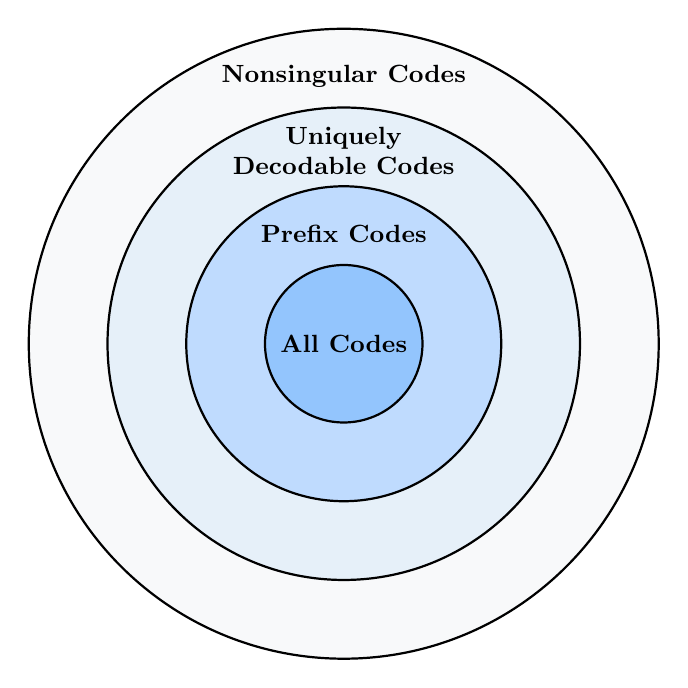
\begin{tikzpicture}[scale=1]
        % Define colors
        \definecolor{outer}{RGB}{248, 249, 250}
        \definecolor{middle1}{RGB}{230, 240, 249}
        \definecolor{middle2}{RGB}{191, 219, 254}
        \definecolor{inner}{RGB}{147, 197, 253}

        % Draw circles from outermost to innermost
        \fill[outer] (0,0) circle (4cm);
        \draw[thick] (0,0) circle (4cm);

        \fill[middle1] (0,0) circle (3cm);
        \draw[thick] (0,0) circle (3cm);

        \fill[middle2] (0,0) circle (2cm);
        \draw[thick] (0,0) circle (2cm);

        \fill[inner] (0,0) circle (1cm);
        \draw[thick] (0,0) circle (1cm);

        % Add labels with proper syntax
        \node[align=center, font=\small] at (0, -0) {\textbf{All Codes}};
        \node[align=center, font=\small] at (0, 1.4) {\textbf{Prefix Codes}};
        \node[align=center, font=\small] at (0, 2.45) {\textbf{Uniquely}\\ \textbf{Decodable Codes}};
        \node[align=center, font=\small] at (0, 3.4) {\textbf{Nonsingular Codes}};   \end{tikzpicture}
    \caption{Hierarchy of different types of codes}
    \label{fig:code-hierarchy}
\end{figure}

\subsection{Prefix Codes}

\textbf{Prefix codes} are codes in which no codeword is the prefix of any other codeword. This property allows for \textbf{instantaneous decoding}—each codeword can be uniquely identified as soon as it is fully received, making it efficient for communication and compression applications. \bigskip

Below are two examples for a binary code \( \mathcal{D} = \{0, 1\}, D = 2 \):

\begin{figure*}
    \centering

    \begin{minipage}{0.4\textwidth}
        \centering
        \begin{tabular}{cc}
            \toprule
            \( x \) & \( C(x) \) \\
            \midrule
            \( a \) & 0          \\
            \( b \) & 100        \\
            \( c \) & 11         \\
            \bottomrule
        \end{tabular}
    \end{minipage}
    \hspace{2cm}
    \begin{minipage}{0.4\textwidth}
        \centering
        \begin{tabular}{cc}
            \toprule
            \( x \) & \( C(x) \) \\
            \midrule
            \( a \) & 00         \\
            \( b \) & 01         \\
            \( c \) & 10         \\
            \( d \) & 11         \\
            \bottomrule
        \end{tabular}
    \end{minipage}

    \bigskip



    \begin{minipage}{0.4\textwidth}
        \centering
        \begin{tikzpicture}[level distance=1.5cm,
                level 1/.style={sibling distance=3cm},
                level 2/.style={sibling distance=1.5cm}]

            % First tree example
            \node (Root1) {Root}
            child {node [label=below:\textbf{0 = a}] {0}} % direct leaf for a
            child {node {1}
                    child {node {0}
                            child {node [label=below:\textbf{100 = b}] {0}}}
                    child {node [label=below:\textbf{11 = c}] {1}}};
        \end{tikzpicture}
    \end{minipage}
    \hspace{2cm}
    \begin{minipage}{0.4\textwidth}
        \centering
        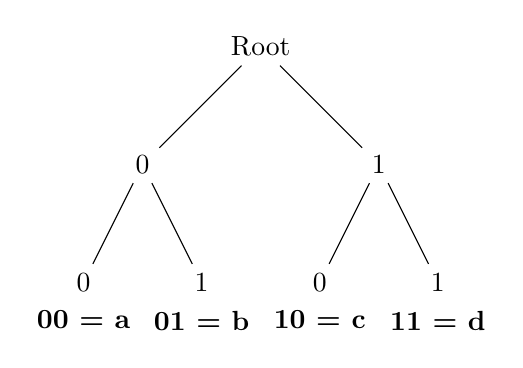
\begin{tikzpicture}[level distance=1.5cm,
                level 1/.style={sibling distance=3cm},
                level 2/.style={sibling distance=1.5cm}]

            % Second tree example
            \node (Root2) {Root}
            child {node {0}
                    child {node [label=below:\textbf{00 = a}] {0}}
                    child {node [label=below:\textbf{01 = b}] {1}}}
            child {node {1}
                    child {node [label=below:\textbf{10 = c}] {0}}
                    child {node [label=below:\textbf{11 = d}] {1}}};
        \end{tikzpicture}
    \end{minipage}
\end{figure*}

\bigskip
\subsubsection{Limits of Prefix Codes}

Prefix codes have constraints related to the structure of the tree. Two key observations are:

\begin{itemize}
    \item A \textbf{complete tree} with \( D^{\ell_{\max}} \) codewords (where \( \ell_{\max} \) is the length of the longest codeword) is fully populated, meaning each branch has reached a leaf at that level.
    \item An \textbf{incomplete tree} has some shorter codewords, reducing the total number of available codewords.
\end{itemize}

Intuitively, adding a new codeword consumes all potential branches (or descendants) that would otherwise be available for longer codewords.

\sn{Key Insight for Prefix Codes}{
    Prefix codes provide efficiency in decoding by ensuring no codeword is a prefix of another– so we do not need a separation character as seen in the Morse Code Example  \ref{ex:morse_code}. However, this comes at the expense of limiting the code length options, as adding a codeword shortens the tree depth for all other codewords.
}


\section{Kraft Inequality}

\thm{Kraft Inequality}{
    The codeword lengths \(\ell_i\) of any \(D\)-ary prefix code must satisfy the inequality:
    \[
        \sum_{i} D^{-\ell_i} \leq 1
    \]
    Conversely, given any set of lengths that satisfy this inequality, there exists a corresponding prefix code.
    \paragraph{Proof:}
    \begin{itemize}
        \item A tree representing a prefix code with the longest codeword length \(\ell_{\text{max}}\) can have at most \(D^{\ell_{\text{max}}}\) leaves.
        \item Each codeword of length \(\ell_i\) corresponds to \(D^{\ell_{\text{max}} - \ell_i}\) descendants at level \(\ell_{\text{max}}\).
        \item Summing over all codewords, the inequality becomes:
              \[
                  \sum_{i} D^{\ell_{\text{max}} - \ell_i} \leq D^{\ell_{\text{max}}} \Rightarrow \sum_{i} D^{-\ell_i} \leq 1
              \]
    \end{itemize}
}


\subsection{Interpretation: Codeword Supermarket}

To illustrate the Kraft inequality, consider the following interpretation. Imagine a “codeword supermarket” where shorter codewords are “more expensive,” and we are constrained by a maximum budget. The inequality \(\sum_i D^{-\ell_i} \leq 1\) reflects the idea that the budget cannot be exceeded.

\begin{marginfigure}[30pt]
    \centering

    \begin{tabular}{|c|c|c|c|l|}
        \hline
        \multirow{8}{*}{0} & \multirow{4}{*}{00} & 000                  & 0000 & \multirow{16}{*}{\rotatebox{90}{The total symbol code budget}} \\
        \cline{3-4}
                           &                     & 001                  & 0001 &                                                                \\
        \cline{3-4}
                           &                     & \multirow{2}{*}{001} & 0010 &                                                                \\
        \cline{4-4}
                           &                     &                      & 0011 &                                                                \\
        \cline{2-4}
                           & \multirow{4}{*}{01} & \multirow{2}{*}{010} & 0100 &                                                                \\
        \cline{4-4}
                           &                     &                      & 0101 &                                                                \\
        \cline{3-4}
                           &                     & \multirow{2}{*}{011} & 0110 &                                                                \\
        \cline{4-4}
                           &                     &                      & 0111 &                                                                \\
        \cline{1-4}
        \multirow{8}{*}{1} & \multirow{4}{*}{10} & \multirow{2}{*}{100} & 1000 &                                                                \\
        \cline{4-4}
                           &                     &                      & 1001 &                                                                \\
        \cline{3-4}
                           &                     & \multirow{2}{*}{101} & 1010 &                                                                \\
        \cline{4-4}
                           &                     &                      & 1011 &                                                                \\
        \cline{2-4}
                           & \multirow{4}{*}{11} & \multirow{2}{*}{110} & 1100 &                                                                \\
        \cline{4-4}
                           &                     &                      & 1101 &                                                                \\
        \cline{3-4}
                           &                     & \multirow{2}{*}{111} & 1110 &                                                                \\
        \cline{4-4}
                           &                     &                      & 1111 &                                                                \\
        \hline
    \end{tabular}

    \caption{visualisation of the Codeword Supermarket}
\end{marginfigure}

\bigskip

\textbf{Note:} While this inequality has been demonstrated for prefix codes, the theorem extends to uniquely decodable codes as well (see MacKay Sec. 5.2 and C\&T Theorem 5.5.1 for further proof), where it guarantees the existence of a set of code lengths that satisfy the condition.

\section{Lagrange Multipliers for Optimal Code Length}

\thm{Theorem: Lagrange Multiplier}{
    Consider a constrained optimisation problem:
    \[
        \min f(\mathbf{x}) \quad \text{subject to} \quad g(\mathbf{x}) = 0
    \]
    where \( \mathbf{x} \in \mathbb{R}^k \), \( f : \mathbb{R}^k \to \mathbb{R} \) is the objective function, and \( g : \mathbb{R}^k \to \mathbb{R}^c \) is the constraint function. \bigskip

    The Lagrangian function for this optimisation problem is defined as:
    \[
        L := f(\mathbf{x}) + \boldsymbol{\lambda} \cdot g(\mathbf{x})
    \]
    where \(\boldsymbol{\lambda}\) represents the Lagrange multipliers. Any local extremum of \( f(\mathbf{x}) \) subject to \( g(\mathbf{x}) = 0 \) satisfies \( \nabla_{\mathbf{x}, \boldsymbol{\lambda}} L = 0 \).
}

In practice, solving a \( k \)-dimensional optimisation problem with \( c \) constraints involves finding \( k + c \) equations as follows:
\begin{itemize}
    \item \( k \) equations for \( x_1, \ldots, x_k \):
          \[
              \frac{dL}{dx_1} = 0, \, \ldots, \, \frac{dL}{dx_k} = 0
          \]
    \item \( c \) equations for \(\lambda_1, \ldots, \lambda_c\):
          \[
              g_1(x) = 0, \, \ldots, \, g_c(x) = 0
          \]
\end{itemize}

\subsection{Optimal Codes}

\hl{How good is the best prefix code for a given $p_i$?}

The objective is to find the best prefix code for a given distribution \( p_i \) by minimising the expected code length:
\[
    \min \sum_i p_i \ell_i \quad \text{subject to} \quad \sum_i D^{-\ell_i} = 1
\]
Using Lagrange multipliers, we define the Lagrangian: \marginnote{
    We make two assumptions: that $l_i$ is continuous, and that the equality constraint is satisfied.}

\[
    L = \sum_i p_i \ell_i + \lambda \left( \sum_i D^{-\ell_i} - 1 \right)
\]

\begin{enumerate}
    \item Differentiate the Lagrangian with respect to \(\ell_i\) and set to 0:
          \[
              \frac{dL}{d\ell_i} = p_i - \lambda D^{-\ell_i} \ln D = 0
          \]
    \item Solve for \(\ell_i\):
          \[
              D^{-\ell_i} = \frac{p_i}{\lambda \ln D}
          \]
    \item Substitute into the Kraft inequality and solve for \(\lambda\):
          \[
              \sum_i D^{-\ell_i} = 1 \Rightarrow \frac{1}{\lambda \ln D} = 1 \Rightarrow \lambda = \frac{1}{\ln D}
          \]
    \item Substitute \(\lambda\) back to obtain the optimal code length:
          \[
              \ell_i^* = -\log_D p_i
          \]
    \item Take the second derivative of the Lagrangian:
          \[
              \frac{d^2L}{d\ell_i^2} = D^{-\ell_i} \ln D \geq 0
          \]
          Since this derivative is non-negative and there is only one solution to \( \frac{dL}{d\ell_i} = 0 \), this solution is a global minimum.
\end{enumerate}

\defb{Entropy is the Optimal Code Length}{
    Thus, the average length of the optimal code is:
    \[
        L^* = \sum_i p_i \ell_i^* = -\sum_i p_i \log_D p_i = H_D(X)
    \]
    which shows that the entropy \( H(X) \) represents the minimum average code length.
}


The above results reveal a duality between probability distributions (PDFs) and prefix codes:
\begin{itemize}
    \item Given a PDF \( p_i \), there exists an optimal code \( C \) with code lengths \( \ell_i = -\log_D p_i \).
    \item Given a set of Kraft-compatible lengths \( \ell_i \), there exists a PDF \( p_i \propto D^{-\ell_i} \) for which these lengths are optimal.
\end{itemize}

These implicit probabilities \( p_i \) are sometimes called the \textbf{implicit probabilities} of the code \( C \).

\section{Huffman Coding}

\thm{Algorithm: Huffman Coding}{
    Huffman coding provides an optimal encoding strategy for a given set of symbols with associated probabilities. The algorithm works as follows:
    \begin{enumerate}
        \item Select the two symbols with the smallest probabilities.
        \item Combine these two symbols into a single "node" and assign it a probability equal to the sum of the original two.
        \item Repeat the above steps until only one node remains.
    \end{enumerate}

    Huffman coding is optimal. That is, if \( C^* \) is the Huffman code and \( C' \) is any other uniquely decodable code, then \( L(C^*) \leq L(C') \).

    \paragraph{Proof: } The proof is complicated, see MacKay, Exercise 5.16, or Cover and Thomas, Sec. 5.8.
}


\subsection{Huffman Coding Example}

Consider an example with symbol set \( X = \{a, b, c, d, e\} \) and probabilities \( p = \{0.25, 0.25, 0.2, 0.15, 0.15\} \).

\begin{figure}

    \centering
    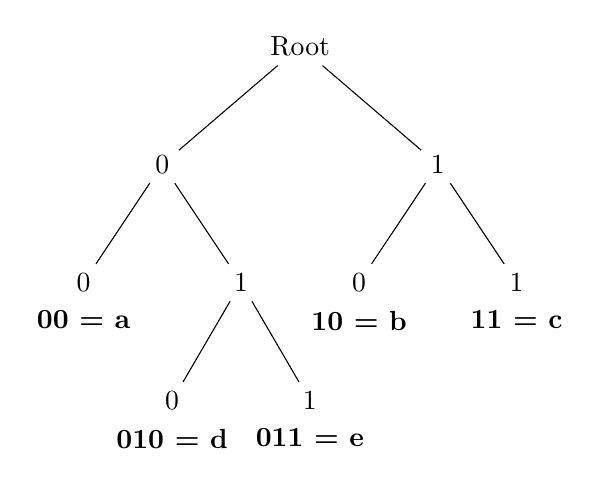
\begin{tikzpicture}[level distance=1.5cm,
            level 1/.style={sibling distance=3.5cm},
            level 2/.style={sibling distance=2cm},
            level 3/.style={sibling distance=1.75cm}]

        % Right-side tree
        \node (Root2) {Root}
        child {node {0}
                child {node [label=below:\textbf{00 = a}] {0}}
                child {node {1}
                        child {node [label=below:\textbf{010 = d}] {0}}
                        child {node [label=below:\textbf{011 = e}] {1}}
                    }
            }
        child {node {1}
                child {node [label=below:\textbf{10 = b}] {0}}
                child {node [label=below:\textbf{11 = c}] {1}}
            };
    \end{tikzpicture}
    \caption{Huffman Tree Example}
\end{figure}




\begin{table}[h!]
    \centering
    \begin{tabular}{ccccc}
        \textbf{Symbol} & \textbf{Probability \( p_i \)} & \textbf{Length \( \ell_i \)} & \textbf{Code \( C(x) \)} \\
        \hline
        \( a \)         & 0.25                           & 2                            & 00                       \\
        \( b \)         & 0.25                           & 2                            & 10                       \\
        \( c \)         & 0.20                           & 2                            & 11                       \\
        \( d \)         & 0.15                           & 3                            & 010                      \\
        \( e \)         & 0.15                           & 3                            & 011                      \\
    \end{tabular}
    \caption{Huffman Coding Example}
\end{table}

In this example, the codewords are assigned by traversing the Huffman tree, with each branch representing either a 0 or a 1.

\sn{Interim Summary: Symbol Codes}{
    \begin{itemize}
        \item Symbol codes map each individual symbol onto a codeword.
        \item Prefix codes are those where no codeword is the start of another codeword, and they can be represented as trees.
        \item \textbf{Kraft inequality}: for prefix codes, \(\sum_{i} D^{-\ell_i} \leq 1\).
        \item \textbf{Source coding theorem for symbol codes}:
              \begin{itemize}
                  \item There exists a code that achieves a length close to \(H(X)\) (achievability).
                  \item There are no codes that achieve length \(< H(X)\) (converse).
              \end{itemize}
    \end{itemize}
}

\section{Using the Wrong Code}

\begin{itemize}
    \item So far, we have assumed a known PDF \( p(x) \) and built a code for it.
    \item What happens if we use the wrong code?

          \ex{Wrong Code}{
              Suppose we assume that the data \( X \) comes from a PDF \( q = \left\{\frac{1}{2}, \frac{1}{4}, \frac{1}{8}, \frac{1}{8}\right\} \) and create a code \( C = \{0, 10, 110, 111\} \) based on this assumption.
              \begin{itemize}
                  \item Expected average length: \( - \frac{1}{2} \log \frac{1}{2} - \frac{1}{4} \log \frac{1}{4} - 2 \times \frac{1}{8} \log \frac{1}{8} = 1.75 \) bits.
                  \item However, if the actual distribution is \( p = \{0, \frac{1}{3}, \frac{1}{3}, \frac{1}{3}\} \), the average length used would be:
                        \[ -0 \log \frac{1}{2} - \frac{1}{3} \log \frac{1}{4} - \frac{2}{3} \log \frac{1}{8} = 2.66 \text{ bits!} \]
                  \item Assuming the wrong distribution means we use more bits than necessary.
              \end{itemize}
          }

\end{itemize}
\marginnote{
    \defsb{Cross Entropy}{
        The cross-entropy of a PDF \( q \) relative to a PDF \( p \) is defined as:
        \[
            H(p, q) := -\sum_{x \in X} p(x) \log q(x)
        \]
        Cross-entropy represents the expected length of a code optimised for \( q(x) \) when applied to samples from \( p(x) \).
    }
}
Mathematically, we can describe the difference in performance as follows:
\begin{itemize}
    \item Consider two random variables on the same alphabet \( X \), with PDFs \( p(x) \) and \( q(x) \).
    \item The optimal code for \( q(x) \) has lengths \( \ell(x) = -\log q(x) \).
    \item When used to compress samples from \( p(x) \), the average length is:
          \[ L(p, q) = \sum_{x \in X} p(x) \ell(x) = -\sum_{x \in X} p(x) \log q(x) \]
\end{itemize}



\section{Kullback-Leibler Divergence}

\defb{Kullback-Leibler Divergence}{
    The Kullback-Leibler (KL) divergence, also known as relative entropy, of two PDFs \( p \) and \( q \) on \( X \) is given by:
    \[
        D_{\text{KL}}(p \parallel q) := \sum_{x \in X} p(x) \log \frac{p(x)}{q(x)}
    \]
    KL divergence measures the "difference" between two distributions.
}

\begin{itemize}
    \item \textbf{Interpretation:} KL divergence quantifies the expected "extra cost" incurred when using a code optimised for \( q \) to compress data that actually follows \( p \).
    \item \textbf{Cross-Entropy Decomposition:}
          \[
              D_{\text{KL}}(p \parallel q) = H(p, q) - H(p)
          \]
          Here, \( H(p, q) \) is the cross-entropy, representing the expected length of the \( q \)-optimal code on \( p \), and \( H(p) \) is the expected length of the \( p \)-optimal code on \( p \).
\end{itemize}
\marginnote{Gibbs' Inequality is extremely important!}

\thm{Gibbs' Inequality}{
    KL divergence is always non-negative:
    \[
        D_{\text{KL}}(p \parallel q) \geq 0
    \]
    Equality holds if and only if \( p(x) = q(x) \) for all \( x \in X \).

    \paragraph{Proof}
    \begin{itemize}
        \item Start with the negative KL divergence:
              \[
                  -D_{\text{KL}}(p \parallel q) = \sum_{x \in \mathcal{X}} p(x) \log \frac{q(x)}{p(x)}
              \]
        \item Using Jensen's inequality, given the concave-down $\cap$ property of the log function:
              \[
                  -D_{\text{KL}}(p \parallel q) \leq \log \sum_{x \in \mathcal{X}} p(x) \frac{q(x)}{p(x)} = \log \sum_{x \in \mathcal{X}} q(x) = \log 1 = 0
              \]
              This leads to the desired result: \( D_{\text{KL}}(p \parallel q) \geq 0 \).
    \end{itemize}

    \paragraph{Proof of Equality condition $(=)$}
    \begin{itemize}
        \item If \( p(x) = q(x) \) for all \( x \in \mathcal{X} \), then:
              \[
                  D_{\text{KL}}(p \parallel q) = \sum_{x \in \mathcal{X}} p(x) \log \frac{p(x)}{p(x)} = \sum_{x \in \mathcal{X}} p(x) \cdot 0 = 0
              \]
              Conversely, since KL is convex in \( q \), it has a unique global minimum, so \( D_{\text{KL}}(p \parallel q) = 0 \) if and only if \( p = q \).
    \end{itemize}


}

\subsection{Properties of KL Divergence}
\begin{itemize}
    \item Why is KL a “divergence”? Let’s consider a \textit{geometric interpretation}.
    \item Due to the convexity of the log function, \( D_{\text{KL}}(p \parallel q) \) is convex in \( q \).
    \item Consider a distribution at a middle point \( \lambda \) between \( p \) and \( q \):
          \begin{align*}
              D_{\text{KL}}\big(p \parallel \lambda q + (1 - \lambda)p\big) & \leq \lambda D_{\text{KL}}(p \parallel q) + (\lambda-1 )\underbrace{D_{\text{KL}}(p \parallel p)}_{= 0} \\
                                                                            & = \lambda D_{\text{KL}}(p \parallel q)
          \end{align*}
\end{itemize}

\begin{center}
    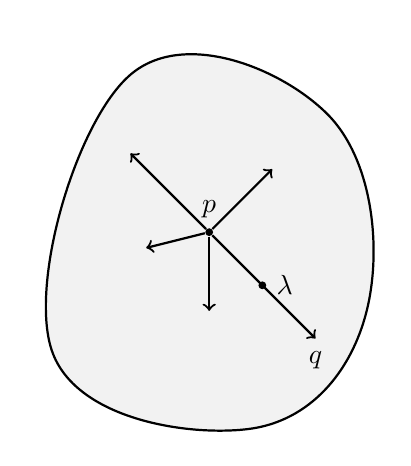
\begin{tikzpicture}
        % Draw curved background
        \draw[thick, fill=gray!10] plot[smooth cycle, tension=0.7] coordinates {(-1,2) (1.5,1.5) (2,-1) (0.5,-2.5) (-2,-1.5)};

        % Draw point p
        \node[circle, fill=black, inner sep=1pt, label=above:$p$] (p) at (0,0) {};

        % Draw point q
        \node[draw=none, inner sep=1pt, label=below:$q$] (q) at (1.35,-1.35) {};

        \node[circle, fill= black, inner sep=1pt, label=right:$\lambda$] (lambda) at (0.675, -0.675) {};

        % Arrows diverging from p
        \draw[->, thick] (p) -- (0.8, 0.8);
        \draw[->, thick] (p) -- (1.35, -1.35);
        \draw[->, thick] (p) -- (0, -1);
        \draw[->, thick] (p) -- (-0.8, -0.2);
        \draw[->, thick] (p) -- (-1, 1);


        % Label for the curved region
    \end{tikzpicture}
\end{center}

\begin{itemize}
    \item The further away you go from \( p \), the larger \( D_{\text{KL}} \) grows.
\end{itemize}

\subsection{KL Divergence as a measure of Entropy}
\marginnote{
    \intuitsb{KL Divergence can be Infinite}{
        If \( q(x) = 0 \) and \( p(x) > 0 \) for any \( x \), then \( D_{\text{KL}}(p \parallel q) = \infty \). \bigskip


        KL becomes infinite if \( p \) contains symbols or events that are not accounted for in \( q \).

    }
}
\begin{itemize}
    \item Entropy can be interpreted as the negative of the KL divergence to a uniform distribution:
          \begin{align}
              D_{\text{KL}}(p \parallel u) & = \sum_i p_i \log \frac{p_i}{u_i} \notag                                                            \\
                                           & = -\sum_i p_i \log \frac{1}{p_i} - \underbrace{\sum_i p_i}_{=1} \log \frac{1}{|\mathcal{X}|} \notag \\
                                           & = -H(P) + \log |\mathcal{X}|
          \end{align}
    \item This property leads to a useful bound on entropy:
          \[
              H(p) = \log |X| - D_{\text{KL}}(p \parallel u) \leq \log |X|
          \]
    \item KL divergence is not symmetric, which makes it unsuitable as a distance metric:
          \[
              D_{\text{KL}}(p \parallel q) \neq D_{\text{KL}}(q \parallel p)
          \]
    \item If \( q(x) = 0 \) and \( p(x) > 0 \) for any \( x \), then \( D_{\text{KL}}(p \parallel q) = \infty \).
\end{itemize}



\ex{Example: KL Divergence Calculations}{
    Given three distributions \( p_1, p_2, \) and \( p_3 \) over the symbols \( a, b, c, d \), with varying probabilities:
    \begin{center}
        % First chart (p1)
        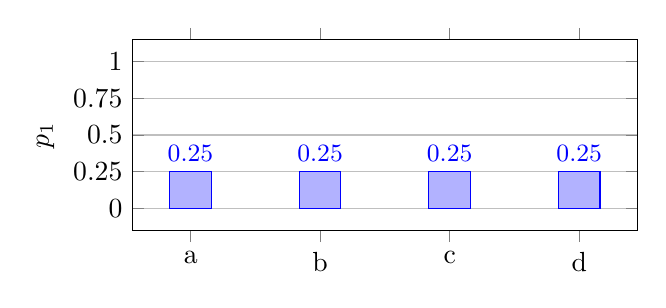
\begin{tikzpicture}
            \begin{axis}[
                    ybar,
                    width=8cm,
                    height=4cm,
                    ymin=0, ymax=1,
                    bar width=15pt,
                    symbolic x coords={a, b, c, d},
                    xtick=data,
                    ylabel={$p_1$},
                    ytick={0, 0.25, 0.5, 0.75, 1},
                    nodes near coords,
                    every node near coord/.append style={font=\small},
                    enlargelimits=0.15,
                    ymajorgrids
                ]
                \addplot coordinates {(a, 0.25) (b, 0.25) (c, 0.25) (d, 0.25)};
            \end{axis}
        \end{tikzpicture}

        % Second chart (p2)
        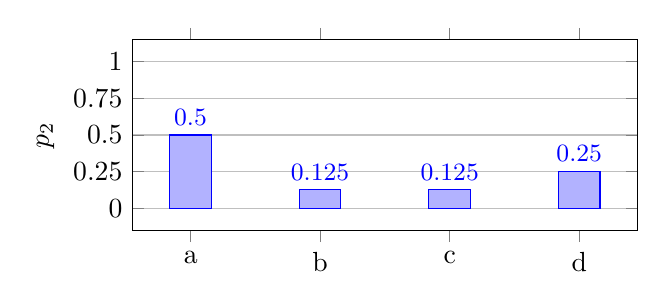
\begin{tikzpicture}
            \begin{axis}[
                    ybar,
                    width=8cm,
                    height=4cm,
                    ymin=0, ymax=1,
                    bar width=15pt,
                    symbolic x coords={a, b, c, d},
                    xtick=data,
                    ylabel={$p_2$},
                    ytick={0, 0.25, 0.5, 0.75, 1},
                    nodes near coords,
                    every node near coord/.append style={font=\small, /pgf/number format/fixed, /pgf/number format/precision=3},
                    enlargelimits=0.15,
                    ymajorgrids
                ]
                \addplot coordinates {(a, 0.5) (b, 0.125) (c, 0.125) (d, 0.25)};
            \end{axis}
        \end{tikzpicture}

        % Third chart (p3)
        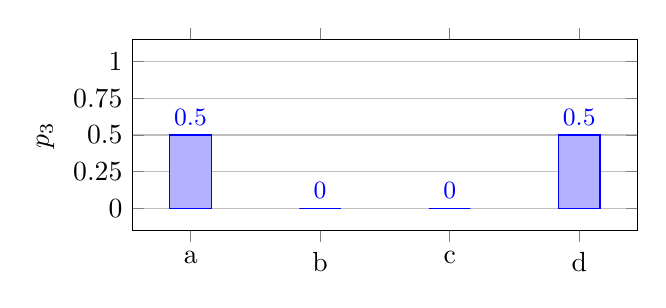
\begin{tikzpicture}
            \begin{axis}[
                    ybar,
                    width=8cm,
                    height=4cm,
                    ymin=0, ymax=1,
                    bar width=15pt,
                    symbolic x coords={a, b, c, d},
                    xtick=data,
                    ylabel={$p_3$},
                    ytick={0, 0.25, 0.5, 0.75, 1},
                    nodes near coords,
                    every node near coord/.append style={font=\small},
                    enlargelimits=0.15,
                    ymajorgrids
                ]
                \addplot coordinates {(a, 0.5) (b, 0) (c, 0) (d, 0.5)};
            \end{axis}

        \end{tikzpicture}

    \end{center}

    \begin{itemize}
        \item \( D_{\text{KL}}(p_1 \parallel p_2) = 0.25 \) bits
        \item \( D_{\text{KL}}(p_2 \parallel p_3) = \infty \) bits (as \( p_3 \) assigns zero probability to some events that \( p_2 \) does not)
        \item \( D_{\text{KL}}(p_3 \parallel p_2) = 0.5 \) bits
        \item \( D_{\text{KL}}(p_3 \parallel p_1) = 1 \) bit
    \end{itemize}
}

% \subsection{KL Divergence in Continuous Distributions}

% To generalise entropy for continuous random variables (RVs), we discretise the domain into bins of width \( \Delta \). For a continuous RV \( X_f \in \mathbb{R} \) with PDF \( f(x) \):
% \[
%     H(X_{f, \Delta}) = -\sum_{i} \Delta f(x_i) \log f(x_i) - \log \Delta
% \]

% Cross-entropy becomes:
% \[
%     H(X_{f, \Delta}, X_{g, \Delta}) = -\sum_{i} \Delta f(x_i) \log g(x_i) - \log \Delta
% \]

% Then, KL divergence is:
% \[
%     D_{\text{KL}}(X_{f, \Delta} \parallel X_{g, \Delta}) = H(X_{f, \Delta}, X_{g, \Delta}) - H(X_{f, \Delta}) = \sum_{i} \Delta f(x_i) \log \frac{f(x_i)}{g(x_i)}
% \]

% Since the \( \log \Delta \) terms cancel, KL remains non-negative in continuous distributions.


\subsection{KL Divergence in Continuous Distributions}

To define entropy in continuous random variables (RVs), we discretise the domain into bins of width \(\Delta\). For a random variable \(X_f \in \mathbb{R}\) with probability density function (PDF) \(f(x)\), the entropy \(H(X^\Delta_f)\) is given by:
\[
    H(X^\Delta_f) = - \sum_i \Delta f(x_i) \log f(x_i) - \log \Delta
\]

Similarly, the cross-entropy \(H(X^\Delta_f, X^\Delta_g)\), where \(g(x)\) is another PDF, is defined as:
\[
    H(X^\Delta_f, X^\Delta_g) = - \sum_i \Delta f(x_i) \log g(x_i) - \log \Delta
\]

By combining these expressions, we obtain the Kullback-Leibler (KL) divergence \(D_{KL}(X^\Delta_f \parallel X^\Delta_g)\) as:
\begin{align*}
    D_{KL}(X^\Delta_f \parallel X^\Delta_g) & = H(X^\Delta_f, X^\Delta_g) - H(X^\Delta_f)                                                                                          \\
                                            & = - \sum_i \Delta f(x_i) \log g(x_i) - \cancel{\log \Delta} - \left(- \sum_i \Delta f(x_i) \log f(x_i) - \cancel{\log \Delta}\right) \\
                                            & = \sum_i \Delta f(x_i) \log \frac{f(x_i)}{g(x_i)}
\end{align*}

Since the terms involving \(\log \Delta\) cancel out, KL divergence remains non-negative in continuous distributions.



% \subsection{KL Divergence for Gaussians}


% Consider two 1D Gaussians \( P \sim \mathcal{N}(\mu_p, \sigma^2_p) \) and \( Q \sim \mathcal{N}(\mu_q, \sigma^2_q) \).

% \begin{itemize}
%     \item Recall the entropy of a Gaussian from previous lectures:
%           \[
%               H(P) = \frac{1}{2} \ln(2\pi e \sigma^2) = \frac{1}{2} \ln(1 + 2\pi e \sigma^2)
%           \]
%     \item To compute the cross-entropy \( H(p, q) = -E_p[\ln q(x)] \):
%           \[
%               H(p, q) = \frac{1}{2} \ln(2\pi \sigma^2_q) + \frac{\sigma^2_p}{2\sigma^2_q} + \frac{(\mu_p - \mu_q)^2}{2\sigma^2_q}
%           \]
%     \item Therefore, KL divergence is:
%           \[
%               D_{\text{KL}}(p \parallel q) = \frac{1}{2} \left( \frac{\sigma^2_p}{\sigma^2_q} - 1 - \ln \frac{\sigma^2_p}{\sigma^2_q} + \frac{(\mu_p - \mu_q)^2}{\sigma^2_q} \right)
%           \]
% \end{itemize}

% This KL divergence grows with the separation of Gaussian means and is larger when Gaussians are narrower and separated further.

\subsection{KL Divergence in Gaussians}

To calculate the Kullback-Leibler (KL) divergence between two one-dimensional Gaussian distributions, let
\[
    P \sim \mathcal{N}(\mu_p, \sigma_p^2) \quad \text{and} \quad Q \sim \mathcal{N}(\mu_q, \sigma_q^2)
\]

We have already derived the entropy of a Gaussian distribution:
\begin{equation}
    H(P) = \frac{1}{2} \ln(2\pi e \sigma^2) \label{eq:gaussian_entropy}
\end{equation}
or equivalently,
\[
    H(P) = \frac{1}{2} (1 + \ln(2\pi \sigma^2))
\]

Now, we calculate the cross-entropy \(H(p, q)\):
\begin{align*}
    H(p, q) & = -\mathbb{E}_p [\ln q(x)]                                                                         \\
            & = \mathbb{E}_p \left[ \frac{1}{2} \ln(2\pi \sigma_q^2) + \frac{(x - \mu_q)^2}{2\sigma_q^2} \right] \\
            & = \frac{1}{2} \ln(2\pi \sigma_q^2) + \frac{1}{2\sigma_q^2} \mathbb{E}_p \left[(x - \mu_q)^2\right]
\end{align*}

To proceed, we evaluate \(\mathbb{E}_p \left[(x - \mu_q)^2\right]\):
\begin{align*}
    \mathbb{E}_p \left[(x - \mu_q)^2\right] & = \mathbb{E}_p \left[x^2 - 2x\mu_q + \mu_q^2\right] \\
                                            & = \mathbb{E}_p[x^2] - 2\mu_p\mu_q + \mu_q^2
\end{align*}

Since \(\sigma^2 = \mathbb{E}[x^2] - \mathbb{E}[x]^2\), we have
\[
    \mathbb{E}_p \left[(x - \mu_q)^2\right]= \sigma_p^2 + \mu_p^2 - 2\mu_p\mu_q + \mu_q^2 = \sigma_p^2 + (\mu_p - \mu_q)^2
\]

Substituting back, the cross-entropy \(H(p, q)\) becomes:
\[
    H(p, q) = \frac{1}{2} \ln(2\pi \sigma_q^2) + \frac{\sigma_p^2}{2\sigma_q^2} + \frac{(\mu_p - \mu_q)^2}{2\sigma_q^2}
\]

Finally, the KL divergence \(D_{KL}(p \parallel q) = H(p, q) - H(p)\) is:
\[
    D_{KL}(p \parallel q) = \frac{1}{2} \left( \frac{\sigma_p^2}{\sigma_q^2} - 1 - \ln \frac{\sigma_p^2}{\sigma_q^2} + \frac{(\mu_p - \mu_q)^2}{\sigma_q^2} \right)
\]

\intuitb{Separation of Gaussians}{
    \begin{center}
        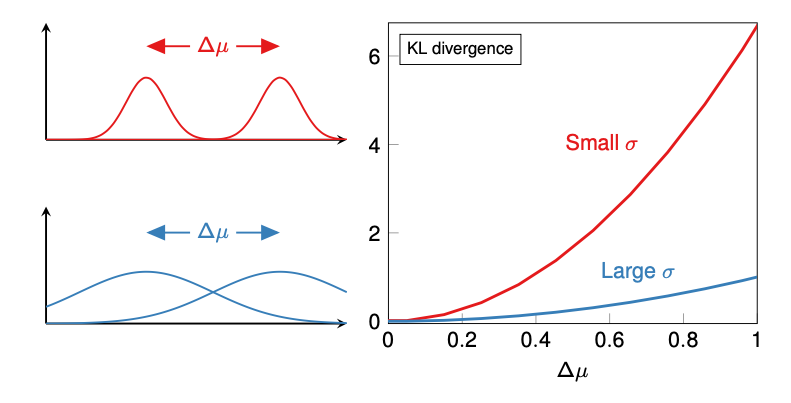
\includegraphics[width=0.9\textwidth]{img/kld_gaussian.png}
    \end{center}
    \begin{itemize}
        \item Consider two Gaussian distributions with \(\sigma_p = \sigma_q\) and let \(\Delta \mu = \mu_p - \mu_q\) represent the difference in their means.
        \item The KL divergence increases more rapidly if two narrow Gaussian distributions (i.e., with smaller variances) are separated further apart in terms of their means.
    \end{itemize}

    So far, we have seen:
    \begin{itemize}
        \item \textbf{Cross-entropy:} Represents the expected code length when using a suboptimal (incorrect) code.
        \item \textbf{KL Divergence:} Measures the difference between two probability distributions and is always non-negative (Gibbs' inequality).
        \item \textbf{Interpretations:}
              \begin{itemize}
                  \item \textit{Compression interpretation:} KL divergence represents the “extra cost” of using an incorrect code.
                  \item \textit{Geometric interpretation:} KL divergence increases as two distributions diverge from each other.
              \end{itemize}
        \item \textbf{Connection to inference:} Minimum code length is mathematically equivalent to maximum likelihood estimation, implying that a good compressor is also a good predictor.
    \end{itemize}

}

\section{Maximum Likelihood Inference}
\defb{Definition: Maximum Likelihood Estimation (MLE)}{Given a dataset \( \mb{x} \) and a family of PDFs \( p(\mb{x}; \theta) \), the maximum likelihood estimate (MLE) of the parameter \( \theta \) is:
    \[
        \theta^*_{\text{MLE}} = \arg \max_{\theta} p(\mb{x}; \theta)
    \]
    MLE is a widely used method in machine learning and data science for estimating model parameters.}


\begin{itemize}
    \item Consider a sample of \( n \) data points \( \mb{x} = \{x_i\}_{i=1}^n \) and a family of probability density functions (PDFs) \( p(\mb{x}; \theta) \) parameterised by \( \theta \).
    \item How do we fit a PDF to $\mb{x}$?


    \item Assuming the data points are independent and identically distributed (i.i.d.), the likelihood of observing \( \mb{x} \) given \( \theta \) is:
          \[
              p(\mb{x}; \theta) = \prod_{i=1}^n p(x_i; \theta)
          \]

    \item It is often convenient to work with the \textbf{log-likelihood function}:
          \[
              L(\theta) = \frac{1}{n} \ln p(\mb{x}; \theta) = \frac{1}{n} \sum_{i=1}^n \ln p(x_i; \theta)
          \]

    \item For large datasets (as \( n \to \infty \)), by the Law of Large Numbers, the log-likelihood converges to the expected value:
          \[
              \lim_{n \to \infty} L(\theta) = \mathbb{E}_p [\ln p(x; \theta)]
          \]
\end{itemize}

\ex{Maximum Likelihood for Gaussian Means}{

    \begin{itemize}
        \item Consider \( n \) i.i.d. data points \( x_1, x_2, \ldots, x_n \) drawn from a Gaussian distribution with unknown mean \( \mu \) and known variance \( \sigma^2 \).

        \item The PDF of each data point under the Gaussian distribution is:
              \[
                  p(x_i; \mu) = \frac{1}{\sqrt{2\pi \sigma^2}} \exp\left(-\frac{(x_i - \mu)^2}{2\sigma^2}\right)
              \]

        \item The log-likelihood function for the mean \( \mu \) is:
              \[
                  L(\mu) = \frac{1}{n} \sum_{i=1}^n \ln p(x_i; \mu) = -\frac{1}{2} \ln(2\pi \sigma^2) - \frac{1}{2n \sigma^2} \sum_{i=1}^n (x_i - \mu)^2
              \]

        \item To find the MLE for \( \mu \), differentiate \( L(\mu) \) with respect to \( \mu \) and set the derivative to zero:
              \[
                  \frac{dL}{d\mu} = \frac{1}{n \sigma^2} \sum_{i=1}^n (x_i - \mu) = 0
              \]

              \begin{center}
                  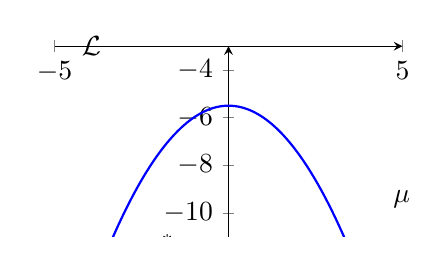
\begin{tikzpicture}
                      \begin{axis}[
                              domain=-5:5,
                              samples=100,
                              axis x line=middle,
                              axis y line=middle,
                              xlabel={\(\mu\)},
                              ylabel={\(\mathcal{L}\)},
                              ymin=-11, ymax=-3,
                              xmin=-5, xmax=5,
                              xtick={-5,0,5},
                              ytick={-10,-8,-6,-4},
                              width=6cm,
                              height=4cm,
                              y label style={at={(axis description cs:0.05,1.1)}},
                              x label style={at={(axis description cs:1.05,0.1)}}
                          ]
                          % Log-likelihood curve
                          \addplot[blue, thick] {-(x^2 / 2) - 5.5};
                          % Vertical line for MLE
                          \addplot[dashed] coordinates {(0,-11) (0,-3)};
                          % MLE label
                          \node at (axis cs:0,-10.5) [anchor=north east] {\(\mu^*_{\text{MLE}}\)};
                      \end{axis}
                  \end{tikzpicture}
              \end{center}

        \item Solving this equation, we obtain:
              \[
                  \mu^*_{\text{MLE}} = \frac{1}{n} \sum_{i=1}^n x_i
              \]
              Thus, the MLE for the mean \( \mu \) is simply the sample mean.
    \end{itemize}
}

\subsection{A Good Compressor is a Good Predictor}

\begin{itemize}
    \item Suppose we have:
          \begin{itemize}
              \item Data \( X \sim p(x) \)
              \item A compressor that uses code lengths \( \ell(x) \)
          \end{itemize}

    \item This means the compressor has learned some certain implicit probabilities \( q(x) \) by setting:
          \[
              q(x) = \frac{1}{z} 2^{-\ell(x)} \quad \text{where} \quad z = \sum_x 2^{-\ell(x)} \quad \text{ and } \ell(x) = -\log z - \log q(x)
          \]

          \(z\) is known as the Kraft number, where the Kraft inequality is satisfied if \( z \leq 1 \).

    \item \hl{By the Source Coding Theorem (SCT), the optimal code length is:
    \[
        \ell^*(x) = -\log p(x)
    \]}


    \item The expected extra cost incurred by using \( q \) instead of the true distribution \( p \) is:
          \begin{align*}
              \mathbb{E}_p [\ell(x) - \ell^*(x)] & = \mathbb{E}_p\left[ -\log x - \log q(x) + \log p(x)\right] \\
                                                 & = \log \frac{1}{z} + D_{KL}(p \parallel q)
          \end{align*}

          where \(\log \frac{1}{z} \geq 0\) by the Kraft inequality. This extra cost is zero iff:
          \begin{itemize}
              \item Kraft eqaulity is achieved, or the `supermarket budget' is spent
              \item The two distributions are the same, i.e., \( p = q \)
          \end{itemize}

          \[
              L = L^* \Leftrightarrow p = q
          \]

    \item Therefore, an optimal compressor has effectively ``learned" the true data distribution.
\end{itemize}

\intuitb{Summary}{
    \begin{itemize}
        \item Symbol codes compress individual symbols, not blocks. Prefix codes are especially useful due to the Kraft inequality and their tree representation.
        \item \textbf{KL Divergence:} Measures the difference between two probability distributions, always non-negative (Gibbs' inequality).
        \item \textbf{Interpretations:}
              \begin{itemize}
                  \item \textit{Compression interpretation:} KL divergence quantifies the “extra cost” of using an incorrect code.
                  \item \textit{Geometric interpretation:} KL divergence increases as two distributions become more dissimilar.
              \end{itemize}
        \item \textbf{Inference connection:} Minimum code length corresponds to maximum likelihood estimation, i.e. a good compressor is a good predictor.
    \end{itemize}
}
